\begin{abstract}
Public videos described as extraterrestrial (ET) channeling circulate through practitioners' accounts, interview programs, and repost channels. Comparing these records requires distinguishing a human speaker from an uploader and a title from spoken content. We present an exploratory, source-linked study of a bounded YouTube index assembled from an existing research atlas and a supplied research archive. The merged sample contains 925 unique upload identifiers; refreshed and explicitly labeled inherited metadata provide 881 usable durations and 880 exact publication dates. We compare sampled upload lengths, transparent keyword indicators, sparse lexical representations, and learned sentence embeddings. A purposive caption pilot retrieves 34 tracks from 36 attempts and retains 30 English documents. In the matched text-layer comparison, 22 videos from 11 publishing accounts contribute to 55 account pairs; title-based and caption-based similarity rankings correlate at only $\rho=0.206$. Name-and-genre masking changes title rankings ($\rho=0.626$), whereas excluding repeated title strings changes them little ($\rho=0.992$). Positionally trimming caption openings and endings preserves broad pair rankings ($\rho=0.969$) but changes four of 13 accounts' nearest neighbors. These descriptive results show that account identity, text layer, and sampling decisions materially affect comparisons in this corpus. They do not assess the origin or truth of channeling claims. We release provenance-preserving metadata, derived features, executable analysis, and an updateable dashboard, while marking human validation and further analyses as TBD.
\end{abstract}

\section{Introduction}
Researchers studying small online communities often encounter material through search results, curated lists, and short titles before obtaining the underlying speech. These layers offer different views of the same record. An uploader may distribute brief extracts, host a practitioner as a guest, or repost an older recording under a new headline. Treating the uploader as the speaker, or the headline as the session, can consequently change the apparent relationships among participants. This is a measurement problem before it is a modeling problem.

ET channeling provides a useful setting in which to examine these distinctions. Public practitioners describe communications attributed to named entities or collectives, while audiences encounter them through recordings, interviews, promotional pages, and community discussion. The Channeling Atlas project initially focused on records associated with Darryl Anka/Bashar, Athina Kr\'ol/Ashtar, and The Galactic Guide/Ryok, then expanded through related names and claimed civilizations. These are attributed identities used to organize public discourse, rather than independently established sources of communication. Our research object is the published record and its computational representation.

The substantive literature contains small prospective studies of channeling, including standardized questions and qualitative analyses \citep{anastasia2020qualitative,wahbeh2023answers,wahbeh2026semantic,wahbeh2026qualitative}. A public-video corpus differs from those designs: speakers answer different questions, uploads vary in length, and the text may include hosts or advertisements. Embedding similarity across such records cannot be read directly as agreement between answers, much less evidence about their attributed origin. At the same time, computational studies of YouTube demonstrate the value of explicitly documented sampling frames and distinguishable channel, video, and content units \citep{ribeiro2021youniverse}. Research on religious YouTube content offers a closer substantive bridge between narrative features and platform presentation \citep{chen2026digital}.

We ask three research questions:
\begin{itemize}
\item \textbf{RQ1:} What coverage and upload-length differences can be established within this bounded index after reconciling its source records?
\item \textbf{RQ2:} How do account comparisons differ between titles and captions when the contributing videos are matched?
\item \textbf{RQ3:} How sensitive are those comparisons to name and genre words, repeated titles, document sampling, and caption boundaries?
\end{itemize}

The contribution is a reproducible measurement study and documented research resource. We audit and merge 925 upload identifiers, retain source precedence and disagreements, and compute account-level statistics with explicit denominators. We execute both a lexical baseline and a pinned learned encoder, alongside an available-caption pilot. We then show that some seemingly similar analytical decisions have different consequences: repeated-string removal is comparatively stable, name-and-genre masking is consequential, and titles weakly preserve the caption-based pair ordering in a small matched cohort. The study supplies a basis for later close reading and human annotation; it does not claim a representative sample, a new embedding algorithm, or a validation of channeling.

\section{Background and Related Work}
\subsection{Channeling as a research object}
The term \emph{channeling} covers heterogeneous practices and attributed sources. Our scope follows the public descriptions attached to discovered records, including adjacent interview and repost accounts; inclusion is not a classification of an individual's private beliefs or a diagnosis. The atlas maintains a separate historical timeline anchored in a Ra-contact focus, with earlier precursors. That archival starting point should not be confused with the historical origin of mediumship or of channeling more broadly.

\citet{anastasia2020qualitative} analyze elicited content from 13 trance channels using qualitative methods. Their design foregrounds the prompt and interpretive context rather than treating an unrestricted collection of utterances as interchangeable observations. \citet{wahbeh2023answers} examine 15 channelers' responses to ten scientist-supplied scientific and metaphysical questions in channeled and non-channeled conditions. The quantitative comparisons involve seven US participants; the qualitative analysis includes those seven and eight Italian participants. The US protocol used a fixed condition order and unequal response-time allowances. The published account reports little cross-channeler correspondence in the quantitative subset, although some qualitative themes overlap. This distinction between shared themes and agreement on answers is directly relevant to our vocabulary and embedding measures.

Two 2026 studies by Wahbeh and Glick examine a three-channeler prospective research program using semantic and qualitative approaches \citep{wahbeh2026semantic,wahbeh2026qualitative}. They motivate comparisons based on equivalent topical prompts and separation of within-person from between-person variation. Our access to these studies includes institutional abstracts, indexed methods, and a public supplement; the publisher full texts were not accessible during this phase. The supplement provides protocol, code, and results artifacts, but does not make the participant answer inputs or all reported analysis components available. We therefore use the studies as design comparators, not as reproduced findings. The two articles are related outputs, not independent replications. Nor can their measures be pooled with the 2023 study or with unstructured YouTube uploads.

An archival channeling study compares two collections through an additional computational layer: both are queried using the same UFODex system, and embeddings compare its generated answers to ten matched questions \citep{wahbeh2026records}. These AI-mediated responses differ from the published titles and available captions analyzed here. The cosine values cannot be pooled, and resemblance in either design does not establish an independent source of information.

Ethnographic accounts place channeling and mediumship in learned practices and audience interactions \citep{klinoron2014channel,tomlinson2019medium}; our access to these two sources was limited to publisher abstracts. A full-text small-community comparator combines twelve Buddhist practitioners' interviews with reflexive thematic analysis and first-author autoethnography \citep{claisse2023faith}. These different settings motivate contextual interpretation, but our public-record analysis lacks participant accounts or equivalent ethnographic grounding. None supplies a classification of our indexed practitioners.

\subsection{YouTube, religion, and small communities}
\citet{ribeiro2021youniverse} document a large English-language YouTube metadata resource and discuss the construction and coverage of a platform dataset. Their scale is different from ours, but the principle transfers: the observable collection process bounds the resulting claims. A source-linked index with hundreds of records is not a random sample merely because all its known identifiers are refreshed.

\citet{chen2026digital} study religious YouTube videos through narrative, visual, and engagement dimensions. This provides a substantive example of connecting platform presentation with religious communication without collapsing every upload into a single topic label. Our study focuses more narrowly on provenance and text-layer comparability; it does not analyze visual content, engagement outcomes, audience interpretation, or religious adherence. Other ICWSM studies use mixed methods to characterize YouTube pathways or content-sharing ecosystems \citep{ota2025pathways,starbird2018ecosystem}. Their methodological lessons concern explicit categories and reuse across publishing surfaces. Their substantive labels, including conspiracy or alternative-media categories, are not transferred to the people in this dataset.

Tube2Vec is a close computational precedent: it encodes titles and descriptions with all-MiniLM-L6-v2, sums their vectors within each video, and averages the 50 most recent videos per account \citep{boesinger2024tube2vec}. It compares content, social-sharing and recommendation representations using task-specific human judgments. Its filtered sample emphasizes large, mostly English accounts. Our contribution concerns matched text layers and sensitivity in a small, selected corpus; averaging account vectors is not itself novel, and Tube2Vec's human validation does not transfer to ours.

\subsection{Text representations and validation}
Automated content analysis requires validation for its intended substantive use \citep{grimmer2013text}. Transparent keyword dictionaries make an early analysis inspectable, but their matches are neither exhaustive topics nor verified meanings. Topic-model evaluation has long distinguished statistical fit from human interpretability \citep{chang2009reading}. More recent work finds that fluent topic descriptions can remain too generic for domain-specific exploration and that human involvement changes their usefulness \citep{li2025haystack}. We consequently describe the nine codebook families as \emph{indicators}, retain their exact regular expressions, and leave blinded human validation as TBD.

Sentence-BERT supports efficient comparison of separately encoded sentences \citep{reimers2019sentencebert}. Embedding benchmarks demonstrate that performance depends on task and language \citep{muennighoff2023mteb,enevoldsen2025mmteb}; an established model cannot be assumed optimal for this discourse. Small-corpus work likewise motivates stability checks rather than treating a single representation as definitive \citep{bloem2019consistency}. We use a small, pinned MiniLM baseline because it can be executed and audited locally. We do not call it state of the art. Contemporary alternatives and topic-model software are recorded in the companion literature register, with preprints distinguished from peer-reviewed publications and reviewed software distinguished from executed software.

Topic-evaluation research further distinguishes statistical coherence, useful interpretation and reliability \citep{doogan2021twaddle,hoyle2021incoherence,schroeder2025reliability}. These constructs require different evidence: interpretable labels need examination against documents, while consistency across fitted-model replications does not establish substantive validity. Our rank correlations describe specific perturbations; they are not the replication-reliability coefficients developed for topic models. Human construct validation remains unfinished.

\section{Data and Provenance}
\subsection{A bounded discovery index}
The original atlas contained 482 unique video identifiers. The supplied Claude archive contained 466 video rows, comprising 457 valid unique video identifiers and nine unlinked leads. Fourteen valid identifiers overlapped the atlas, yielding $482+457-14=925$ unique uploads. The archive's video listings were frequently capped near 30 records. Its 92 directory rows included only 53 actual account routes; collection-credit exhaustion explained some absent routes. Missing records were therefore not treated as evidence that an account or practitioner did not exist.

The underlying discovery process used public names, claimed entity/civilization terms, platform searches, linked websites, and community leads. It was purposive and evolved during the project. The frame also includes adjacent non-ET spiritual/contextual uploads, so not every record is independently verified as an ET-channeling performance. The present analysis refreshes and compares that frozen union; it does not retroactively convert discovery into a preregistered search protocol. We do not estimate the total number of active mediums or the probability that an account was included. Older uploads, adjacent interview programs, and repost accounts remain because they help interpret the published record.

\subsection{Units and source precedence}
We distinguish five units: a human practitioner, a publishing account, a YouTube upload identifier, an original session, and a text document. A sixth field records an attributed entity label. These units can have many-to-many relationships. One human can appear on multiple accounts; one account can host multiple speakers; one session can be edited into many upload identifiers. Unique upload IDs remove exact URL duplication, not duplicate performances.

The metadata pass processed every identifier in the union on 23 October 2026 through unauthenticated watch-page requests with five concurrent workers, without cookies, proxies, media downloads, or retries. Request-start times ranged from 19:24:24.900490 to 19:36:49.426737 UTC; the frozen receipt was created at 19:37:52.190727 UTC. These are request-start times, not measured response-completion times. The procedure specified stopping on HTTP 403 or 429; neither occurred. It obtained usable metadata for 878 identifiers and recorded 47 unsuccessful retrieval outcomes. A visible metadata record does not establish that a video can be played without payment or authentication. Positive durations were retrieved for 877 uploads; four inherited positive durations remain explicitly labeled, yielding 881 analyzed durations. The 878 freshly observed exact dates and two inherited dates yield 880 dated records. Publication timestamps may date a repost rather than the original session and do not establish recent practitioner activity. Relative-age strings remain separate text and are never converted into invented exact days. Current timestamps are represented as UTC dates; one-day differences from earlier records may reflect time-zone conventions.

Fresh watch metadata takes precedence for title, uploader binding, duration, and date. Supplied titles, including localized variants, remain in provenance fields. This matters when a practitioner appears as a guest: a Brad Johnson interview, for example, belongs to its observed uploader rather than automatically to Johnson's own account. The complete directory retains 256 route groups, including unresolved or empty historical leads; 180 groups have at least one attributed upload and 178 have measured durations. These figures are account-group counts, not counts of unique mediums.

\begin{table}[t]
\centering
\begin{tabular}{@{}lr@{}}
\toprule
Measure & Count \\
\midrule
Unique indexed videos & 925 \\
Public watch metadata retrieved & 878 \\
Known durations (fresh / inherited) & 881 (877 / 4) \\
Exact publication dates & 880 \\
Videos attributed to account routes & 886 \\
English-likely titles / embedded titles & 742 / 706 \\
Title publishers with $n\geq5$ & 23 \\
Caption attempts / retrieved tracks & 36 / 34 \\
English caption pilot / publishers & 30 / 17 \\
Caption comparison videos / publishers & 26 / 13 \\
Matched eligible / contributing videos & 25 / 22 \\
Matched publishers / dependent pairs & 11 / 55 \\
\bottomrule
\end{tabular}

\caption{Coverage within the frozen index. Each row has its own unit and denominator; no row estimates a platform-wide population. Caption and matched-comparison subsets are described separately in the text.}
\label{tab:coverage}
\end{table}

\subsection{Titles and the caption pilot}
The primary title analysis retains English-likely strings with at least four alphabetic words and a \texttt{langdetect} probability of at least 0.80, using version 1.0.9 with seed 42. These are heuristic decisions, not human language labels. The gate retains 742 titles; 706 have publisher attribution and receive embeddings. The account-level title comparisons require at least five eligible titles, leaving 23 groups. Very short titles and localized titles are especially vulnerable to language-classification error.

The caption pilot selected the first two valid IDs in each supplied status-ok account listing, supplemented by the focal Bashar and Athina Kr\'ol accounts, and excluded explicit donation, registration, and all-day-event titles. The supplied order was not independently established as a complete reverse-chronological enumeration. The Aluna Ash listing contained only one entry; an additional Scranton upload supported the separate concordance case. This procedure selected 36 uploads across 18 practitioner/publisher groupings. Caption acquisition used youtube-transcript-api 1.2.4; records preserve the date 23 October 2026 but not a time of day. Available tracks were retrieved for 34 uploads: 32 automatic and two platform-labeled manual tracks across the full retrieved set. The manual label indicates a non-auto-generated track, not proof of human transcription or verification. The main analysis retains 30 English documents (28 automatic and two platform-labeled manual) from 17 publishing groups after excluding three non-English tracks and one additional concordance case. Thirteen groups have two eligible documents; four have one. Account-level caption similarity uses the 13 groups meeting the two-document threshold. This small selected set supports a feasibility and measurement analysis, not a survey of all available channeling speech.

For matched title/caption indicators, 25 pilot videos also have eligible attributed titles. For matched account centroids, the additional two-document rule leaves 11 accounts and 22 contributing videos. Thus the vocabulary-presence comparison uses 25 videos, while the account-pair ranking comparison uses 55 pairs derived from 22 videos. Keeping these denominators separate prevents a larger eligibility pool from being mistaken for the effective comparison sample.

Figure~\ref{fig:coverage} summarizes the separate selection sequences. No caption was translated, audio-corrected, or speaker-diarized. Hosts, questions, advertisements, and promotional speech can remain. One unavailable pilot track had captions disabled and another was members-only; those access limitations were retained rather than circumvented. Full caption text and retrieved author-page text are not redistributed with this release.

\begin{figure*}[t]
\centering
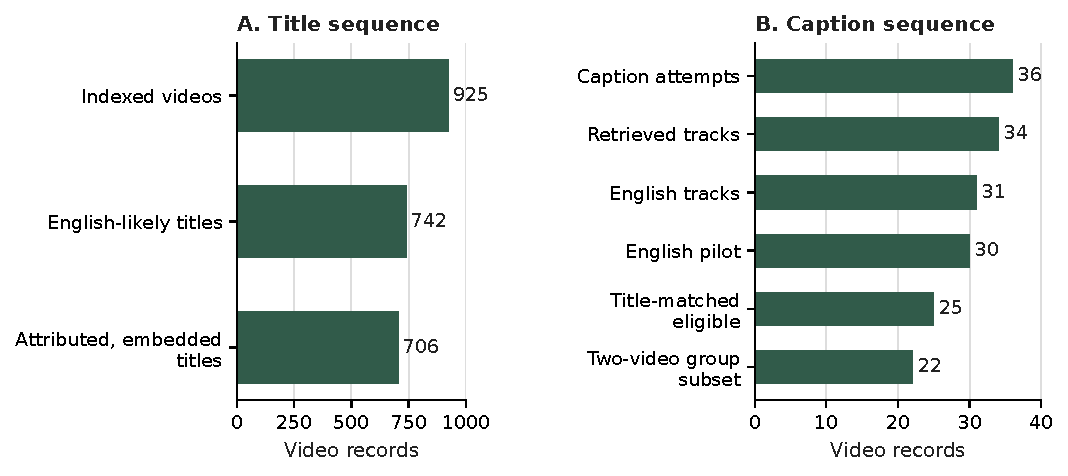
\includegraphics[width=\textwidth]{generated/figures/coverage.pdf}
\caption{Separate title and caption selection sequences. The two panels have different scales and denominators. English-language detection on titles differs from caption-track language labels. In the caption panel, one supplementary English concordance case is excluded from the 30-document pilot; 25 videos pass matched-title eligibility, and 22 contribute to account comparisons after excluding singleton groups.}
\label{fig:coverage}
\end{figure*}

\section{Analytical Methods}
\subsection{Lengths, dates, and transparent indicators}
For publishing group $c$, let $V_c$ be its indexed uploads and $D_c\subseteq V_c$ those with usable duration. We report $|D_c|/|V_c|$, the arithmetic mean, median, and linearly interpolated 25th and 75th percentiles over $D_c$. Missing durations are null, never zero. The quartile interval summarizes the observed uploads; it is not a confidence interval. Monthly counts use only exact-date records and describe the index, not a complete account posting schedule.

Nine overlapping keyword families cover contact/disclosure; choice/beliefs/manifestation; healing/wellbeing; consciousness/awakening; energy/frequency; collective/world events; love/relationships; meditation/practice; and time/dimensions/realities. A title indicator is the proportion of eligible titles with at least one case-insensitive regular-expression match. Caption rates instead count occurrences and normalize each video before averaging:
\begin{equation}
 R_{ct}=\frac{1}{|C_c|}\sum_{v\in C_c}\frac{1000\,m_{vt}}{w_v},
\end{equation}
where $m_{vt}$ is the number of matches for indicator $t$, $w_v$ is the number of tokens matching \texttt{[A-Za-z]+(?:'[A-Za-z]+)?}, and $C_c$ is the included caption set. Contractions count as one token. Indicators overlap; rates need not sum to 1,000. This calculation uses the original caption text, while the embedding pipeline separately masks the predefined name and genre terms. Caption presence and title presence are not equivalent measures of thematic emphasis because captions provide far more opportunities to match a word.

\subsection{Lexical and learned representations}
The lexical baseline uses name-and-genre-masked English word unigrams and bigrams with TF--IDF, sublinear term frequency, minimum document frequency 2, and maximum document frequency 0.9. Account vectors are normalized means of document vectors. This baseline measures shared vocabulary and is kept distinct from a neural semantic representation.

The learned encoder is \texttt{sentence-transformers/all-MiniLM-L6-v2}, pinned to revision \texttt{1110a243fdf4706b} (prefix; full revision and artifact hashes in the model manifest). It produces 384-dimensional vectors using the recorded ONNX artifact and tokenizer. Attention-mask mean pooling includes the unpadded sequence positions; vectors are $L_2$ normalized. Titles use at most 254 wordpieces plus special tokens. Captions are divided into non-overlapping 240-wordpiece chunks, avoiding silent truncation to the first passage. Let $z_{vk}$ be a normalized chunk vector, and let $\mathcal{N}(x)=x/\|x\|_2$. The document and account vectors are
\begin{equation}
 e_v=\mathcal{N}\!\left(\frac{1}{K_v}\sum_{k=1}^{K_v}z_{vk}\right),\qquad
 a_c=\mathcal{N}\!\left(\frac{1}{|C_c|}\sum_{v\in C_c}e_v\right).
\end{equation}
Cosine similarity is $s(c,d)=a_c^\top a_d$. Equal video weighting prevents longer recordings from contributing more chunks to the account representation. Equal chunk weighting gives a short final chunk the same weight as a full chunk, a choice tested below. Name-and-genre masking removes a documented set of practitioner/entity names and generic genre or packaging terms and is evaluated against an unmasked-title condition. Neither masking nor normalization removes all genre, speaker, or promotional effects.

\subsection{Sensitivity and matched comparisons}
All analyses are retrospective and exploratory. We compare pair orderings with Spearman correlation on the intersection of eligible unordered account pairs. Pairwise similarities reuse documents and are dependent, so we do not interpret the number of pairs as a sample size for conventional independent-observation inference. We report no confirmatory $p$-values or population confidence intervals.

Five perturbations examine specific choices. First, raw and name-and-genre-masked titles test sensitivity to names and generic genre/packaging vocabulary. The mask includes terms such as channel, transmission, message, official, galactic, and council; names and generic terms were not separately ablated. Second, we exclude every document whose normalized masked title string is repeated; this is a narrow duplicate-string sensitivity, not original-session deduplication. Third, 50 seed-42 repetitions sample five titles without replacement per eligible account and record the most frequently selected nearest account. The resulting repeat share describes this resampling procedure, not a probability of a true relationship. Fourth, we remove the first and last floor(0.10 times the token count) whitespace-separated tokens after masking from each caption and recompute representations. This trimming tokenizer differs from the alphabetic-token keyword denominator. The positional operation does not identify speakers or isolate an attributed voice.

Fifth, a targeted pooling check keeps the caption text, tokenizer, model and chunks fixed while weighting chunk $k$ by its number $m_{vk}$ of content WordPieces, excluding special tokens:
\begin{equation}
 \widetilde e_v=\mathcal{N}\!\left(\frac{\sum_{k=1}^{K_v}m_{vk}z_{vk}}{\sum_{k=1}^{K_v}m_{vk}}\right).
\end{equation}
Account centroids still give each video equal weight. This changes the influence of a short terminal chunk without changing speaker composition or document selection.

The matched analysis computes title and caption centroids from exactly the same videos in each eligible account. The paper extension additionally removes one publishing account at a time from this matched pair set and recomputes the rank correlation. This leave-one-account-out range is an influence diagnostic on the selected accounts. It does not correct the original sampling bias or create independent observations.

\section{Results}
\subsection{RQ1: Coverage improves, while upload formats remain heterogeneous}
Combined current and labeled inherited metadata provide usable duration for 95.2\% of the 925 indexed uploads and an exact date for 95.1\%. These totals include four inherited durations and two inherited dates. This is high coverage within the index, not high coverage of YouTube. The unresolved remainder, empty account routes, and inherited observations remain visible in the data and dashboard. Source checks also replace localized title variants and correct guest/uploader attribution without discarding the earlier evidence.

\begin{table*}[t]
\centering
\begin{tabular}{@{}lrrrrr@{}}
\toprule
Publisher & Known / indexed & Mean & Median & $Q_1$--$Q_3$ & $\geq30$ min \\
\midrule
Bashar (official) & 16 / 16 & 3.4 & 3.1 & 2.0--4.7 & 0\% \\
Athina Król & 9 / 9 & 40.6 & 47.2 & 24.5--53.4 & 67\% \\
The Galactic Guide & 34 / 34 & 16.6 & 17.0 & 14.7--19.5 & 0\% \\
RIZ \& Lady O & 30 / 30 & 20.6 & 6.0 & 3.6--16.2 & 23\% \\
Lorie Ladd & 30 / 30 & 42.4 & 33.2 & 13.8--73.7 & 53\% \\
Divine Insights & 22 / 22 & 170.3 & 134.0 & 118.5--248.3 & 86\% \\
Bashar Channeling Podcast & 20 / 21 & 103.5 & 88.0 & 73.6--148.2 & 100\% \\
Daniel Scranton & 35 / 35 & 19.8 & 15.6 & 14.2--18.9 & 11\% \\
\bottomrule
\end{tabular}

\caption{Selected publishing accounts emphasized in the research brief. Durations are minutes; $n/N$ is measured/indexed uploads. Means and medians describe these samples. Selection is illustrative, not a ranking. Full quartiles and all groups are in the released CSV.}
\label{tab:duration}
\end{table*}

The focal examples in Table~\ref{tab:duration} and Figure~\ref{fig:duration} show why a single pooled average would be uninformative. The sampled official Bashar account averages 3.4 minutes, whereas the sampled Bashar Channeling Podcast account averages 103.5 minutes. Athina Kr\'ol's nine sampled uploads average 40.6 minutes and The Galactic Guide's 34 average 16.6 minutes. These observations suggest that extracts and longer-format uploads deserve separate annotation; they do not themselves constitute a validated format taxonomy. A mean above the median shows that longer uploads influence the sample average, not that an account is more active or substantive.

\begin{figure*}[t]
\centering
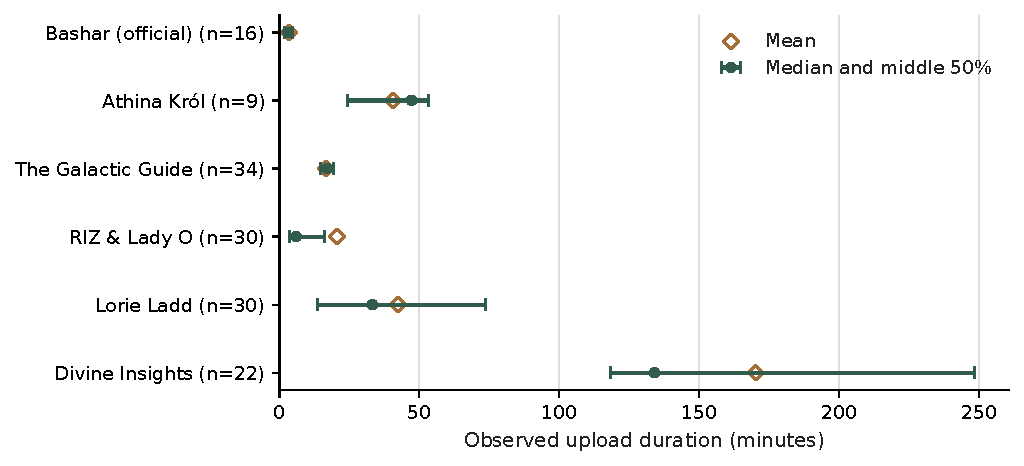
\includegraphics[width=\textwidth]{generated/figures/duration.pdf}
\caption{Observed upload lengths for six illustrative accounts. Green dots mark medians, whiskers the middle 50\%, and orange diamonds means; labels give the number of measured uploads. The quartile spans describe observed durations and are not confidence intervals. These are convenience samples, not complete account histories.}
\label{fig:duration}
\end{figure*}

\subsection{RQ2: Titles weakly preserve the matched caption ordering}
Figure~\ref{fig:matched} shows the matched text-layer comparison and account-omission diagnostic. For the 11 eligible matched accounts, title-based and caption-based similarity rankings correlate at $\rho=0.206$ across 55 pairs. Matching the contributing 22 videos removes one important alternative explanation---different videos on each side---but it does not remove text-length, editing, recognition, or genre differences. This result is therefore evidence about the representations of this pilot, not a universal estimate of how informative video titles are.

The matched vocabulary-presence comparison, using the broader 25-video eligible pool, reinforces the difference in observation opportunity. For example, choice/belief/manifestation keywords appear in three titles but 23 captions; contact/disclosure keywords appear in four titles and ten captions. These are dictionary matches. Their difference cannot be interpreted as a validated theme prevalence or as the proportion of a session devoted to a topic. Longer captions naturally offer more chances for any keyword to occur.

\begin{figure*}[t]
\centering
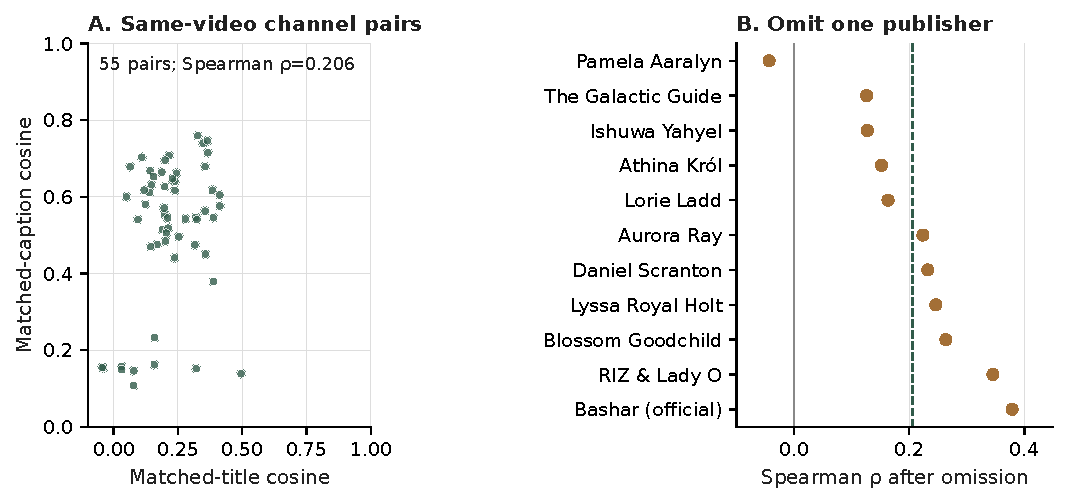
\includegraphics[width=\textwidth]{generated/figures/matched-similarity.pdf}
\caption{Matched text-layer comparison and publisher-omission sensitivity. (A) Both representations use the same 22 videos from 11 accounts, yielding 55 dependent pairs. (B) Each point omits one account and its incident pairs; the dashed line marks the full-pilot rank correlation. The omission range is an influence diagnostic, not a confidence interval. Scores are text resemblance, not probabilities.}
\label{fig:matched}
\end{figure*}

Within the full 30-document caption pilot, the median cosine is 0.661 for 13 same-publisher video pairs and 0.431 for 422 different-publisher pairs. The groups overlap and pairs are dependent. Publisher-specific vocabulary, host speech, repeated prompts, formatting, and recording length are all plausible contributors. The comparison neither identifies a stable speaker signature nor distinguishes an attributed entity's voice from other speech.

\subsection{RQ3: Different perturbations expose different instabilities}
\begin{table*}[t]
\centering
\begin{tabular}{@{}lrrr@{}}
\toprule
Comparison & Publishers & Pairs & Spearman $\rho$ \\
\midrule
Raw vs name-and-genre-masked titles & 23 & 253 & 0.626 \\
All vs deduplicated titles & 23 & 253 & 0.992 \\
Full vs positionally trimmed captions & 13 & 78 & 0.969 \\
Matched titles vs matched captions & 11 & 55 & 0.206 \\
Equal-chunk vs token-weighted captions & 13 & 78 & 0.984 \\
\bottomrule
\end{tabular}

\caption{Descriptive rank-order sensitivity. Correlations compare aligned unordered account-pair scores, not independent observations. The matched text-layer comparison is a different measurement contrast from the four perturbation comparisons in the table.}
\label{tab:sensitivity}
\end{table*}

Figure~\ref{fig:sensitivity} places the perturbations beside the caption-length distribution. Raw versus name-and-genre-masked title rankings correlate at 0.626 across 253 pairs, showing that the selected name and genre vocabulary materially affects the account ordering. Excluding ten documents with repeated normalized masked title strings produces a much higher correlation of 0.992. This stability applies only to exact normalized title repetition; differently titled edits of the same performance can remain.

Caption boundary trimming produces a correlation of 0.969 across 78 account pairs, with median absolute score change 0.022. Yet the nearest account changes for four of the 13 eligible accounts: Athina Kr\'ol, Daniel Scranton, Wendy Kennedy's publishing group, and Pamela Aaralyn. A high global rank correlation therefore coexists with unstable individual neighbor labels. Trimming also leaves interior host speech and promotion untouched. It should not be presented as a test of a purified channeling voice.

\paragraph{Publisher-omission sensitivity.}
The matched title--caption comparison contains \AtlasNMatchedEligibleVideos{} eligible videos, of which \AtlasNMatchedContributingVideos{} contribute to the publisher-level comparison because their \AtlasNMatchedPublishers{} publishers each have at least two records. The resulting \AtlasNMatchedPairs{} off-diagonal pairs give Spearman $\rho=\AtlasRhoMatched$. Removing one publisher and all of its incident pairs leaves ten publishers and 45 pairs. Across the eleven deterministic omissions, the correlation ranges from \AtlasLopoMin{} (omitting Pamela Aaralyn Channeling) to \AtlasLopoMax{} (omitting the official Bashar account). This range describes sensitivity to the included publishers; it is neither a confidence interval nor evidence of a statistically established positive or negative association. The pair values share publishers and videos and are not independent observations.

\paragraph{Caption-length heterogeneity.}
The \AtlasNCaptionPilot{} English-pilot caption documents contain \AtlasCaptionWordsTotal{} word tokens in total. Lengths range from \AtlasCaptionWordsMin{} to \AtlasCaptionWordsMax{}, with median \AtlasCaptionWordsMedian{} and linear first and third quartiles of 579 and 2,546.25 tokens. The shortest document is from hgrfrequencies and the longest from Lorie Ladd. This nearly 99-fold range motivates chunking within videos and equal weighting across videos when constructing publisher centroids. It does not establish the relative amount of channeling speech: captions also contain hosts, audience questions and promotional material, and their word counts reflect the specified tokenizer and available caption track.

\paragraph{Chunk-weighting sensitivity.}
The same \AtlasNCaptionPilot{} caption documents produce \AtlasNContentWordpieces{} content WordPieces in \AtlasNWordpieceChunks{} nonoverlapping chunks, with \AtlasChunksMin{}--\AtlasChunksMax{} chunks per video. The equal-chunk replay reproduces every published video-vector coordinate within $7.5\times10^{-9}$. Weighting each chunk by its content-token count, while retaining equal-video publisher aggregation, yields rank correlation $\rho=\AtlasRhoChunkWeighted$ over the same 78 off-diagonal pairs among 13 two-video publishers (26 contributing documents). Mean and maximum absolute cosine changes are \AtlasChunkCosineMeanChange{} and \AtlasChunkCosineMaxChange{}, respectively. Nearest-neighbor identities change for \AtlasChunkNeighborChanges{} of 13 publishers: Daniel Scranton changes from Blossom Goodchild to RIZ \& Lady O; Pamela Aaralyn changes from Elsa Farrus to Lorie Ladd. This targeted intervention demonstrates sensitivity of local comparisons to how a short final chunk is weighted; it does not establish that either pooling choice measures true thematic similarity.


\begin{figure*}[t]
\centering
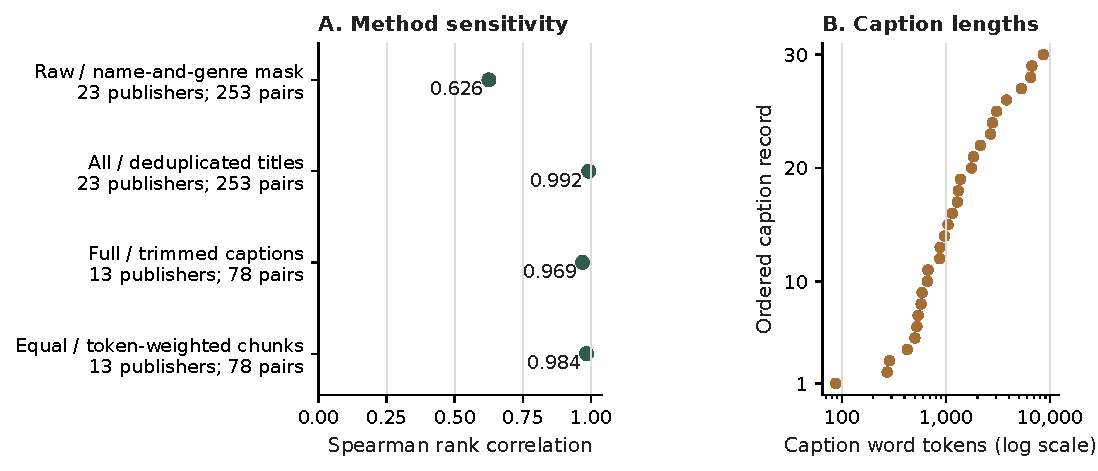
\includegraphics[width=\textwidth]{generated/figures/sensitivity.pdf}
\caption{Sensitivity and caption lengths. (A) Rank correlations compare aligned account-pair scores under four distinct perturbations. Pair counts are not independent sample sizes. (B) The 30 English-pilot caption documents sorted by alphabetic-word count on a logarithmic horizontal scale. Length reflects all available captioned speech, including unseparated hosts and promotion.}
\label{fig:sensitivity}
\end{figure*}

\section{Discussion}
\subsection{Publishing accounts and text layers are substantive choices}
The main result is not that one account is ``closest'' to another. It is that the answer changes with the object being compared. A title centroid describes how indexed uploads are presented. A caption centroid describes the available speech in selected recordings, including other speakers and promotional material. An account grouping describes distribution, whereas a human-medium grouping would require an additional, evidence-backed attribution task. These distinctions should inform both computational summaries and qualitative interpretation.

The weak matched title/caption ordering motivates a practical sequence for further work. Titles can support discovery and visible framing analysis. Claims about spoken themes require captions or licensed transcripts, and claims about agreement require contextual units and human interpretation. When title and caption similarities disagree, the disagreement is a cue to inspect the records, not an error to erase by selecting a preferred model.

\subsection{Small-corpus similarity requires local validation}
The sensitivity results do not justify an all-purpose robustness label. Name-and-genre masking, repeated-string exclusion, and boundary trimming perturb different things. A stable rank ordering after one perturbation does not imply stability under speaker segmentation, translation, a new encoder, or new accounts. Likewise, a low repeat share in a balanced five-title sample describes limited support for a particular nearest-neighbor label under that procedure, not unreliability of a person's communications.

One supplementary concordance case illustrates the need for segmentation. An official Daniel Scranton page links the exact sampled video. Ordered token matches cover 96.7\% of the written message but only 42.5\% of its caption tokens under the supplementary Unicode-word alignment. In a separate caption-observed closing-window calculation, 52.2\% of alphabetic words occur after the closing. These denominators use different, documented tokenizers. The case does not validate recognition accuracy across the corpus; it shows that a whole upload can contain substantial material beyond the attributed message.

Future close reading should select contrasting pairs and account for prompts, voices, and text length. Human annotators could distinguish topical overlap, semantic agreement, disagreement, and reusable formulae. The prospective channeling studies suggest the value of matched questions, but the current observational corpus cannot reproduce that experimental control retrospectively. A better model alone would not solve this design difference.

\subsection{An updateable research resource}
The dashboard makes per-account averages, coverage, dates, indicators, and source-linked observations inspectable. Each analytical release is tied to hashes of its inputs, model artifacts, and generated features. Earlier round snapshots and correction records remain available rather than being silently overwritten. The manuscript's tables and figures are generated from frozen evidence so that later corpus expansion can be accompanied by an explicit change log.

We distinguish two reproduction modes. The public offline mode recalculates descriptive statistics and lexical features, then checks the fingerprint of frozen neural derivatives. A full neural recomputation additionally requires the pinned model and locally available authorized caption text. Numeric embedding archives do not substitute for the missing source text, and public reproducibility of derived calculations is not the same as unrestricted redistribution of speech.

\section{Limitations, Ethics, and Researcher Responsibility}
The index is purposive, English-biased, historically mixed, and influenced by platform visibility and prior search choices. Inclusion probabilities are unknown. The number of account groups cannot support a worldwide active-medium count, and a complete refresh of known IDs cannot establish a complete account history. Same-session reposts remain unresolved. Some account routes are historical or ambiguous; public source precedence resolves only observed conflicts.

The caption pilot is small and selected. Automatic recognition errors, missing tracks, multiple speakers, and unequal text lengths can affect every downstream representation. Language detection is particularly uncertain for short titles. Dictionary families are overlapping and unvalidated; the name-and-genre-mask list is a researcher decision; the encoder is an English baseline without in-domain human evaluation. The chunk-weighting sensitivity test checks one pooling alternative, while thresholds and other model choices remain additional decisions. The leave-one-account-out analysis is an influence diagnostic, not a remedy for selection bias. No causal or ontological conclusion follows from these similarities.

The study uses public professional publishing records and documents attributed claims without affirming or diagnosing them. It does not seek private contact information, private group membership, or access-controlled speech. Caption-disabled and members-only outcomes are recorded as limitations. Public availability does not remove copyright or contextual privacy concerns: raw caption and author-page bodies are excluded from the distributable package. No audience-level targeting or psychological classification is performed. Any future participant interviews or human annotation involving sensitive data require an appropriate institutional determination before collection.

\textbf{TBD: institutional ethics determination, human authorship and affiliations, contributor approval, and release-rights review.} No ethics-board approval, consent procedure, preregistration, or independent human peer review is claimed. This is a working research draft, not a submitted or accepted ICWSM paper. The venue's current formatting and research-ethics guidance informs its organization; compliance must be checked again for a concrete submission.

\section{Conclusion}
This exploratory study makes the observational unit and text layer visible in a public-video analysis of ET channeling discourse. Source reconciliation substantially improves coverage within the 925-upload index, while account-level duration summaries reveal strongly different sampled upload lengths. A small matched caption pilot shows that title-based similarity weakly preserves caption-based pair ordering, and sensitivity tests show why global stability should not be equated with stable nearest neighbors. The reusable contribution is the linked evidence, explicit measurement choices, and executable analysis. Human interpretation, broader sampling, and better speaker/context annotation remain necessary before extending these results to substantive agreement or population-level claims.

\section*{Generative AI and Review Disclosure}
This working draft, analysis code, figures, and accompanying dashboard were prepared with an AI assistant and six model-agent workstreams covering provenance, corpus acquisition, methods, implementation, literature, and presentation. Three analysis rounds preceded publication of the dashboard; three further manuscript rounds are recorded in the paper's review directory. The agents reconstructed numerical outputs and inspected sources and rendered artifacts, but are not independent human reviewers or authors. Human author review, factual acceptance, and accountability are \textbf{TBD}. For a future double-blind submission, the placement and wording of this disclosure must be reconciled with current venue instructions.

\bibliography{references}

% Questions transcribed from the unchanged official-linked PDF in vendor/.
% All answers are intentionally TBD. This is not a completed submission checklist.
% Place immediately after references and before \appendix.
\section*{Paper Checklist}
\noindent\textbf{Working draft: every answer below requires human author review.}
\newcommand{\ChecklistTBD}{\textbf{TBD}}
\begin{enumerate}
\item For most authors...
\begin{enumerate}
\item Would answering this research question advance science without violating social contracts, such as violating privacy norms, perpetuating unfair profiling, exacerbating the socio-economic divide, or implying disrespect to societies or cultures? \ChecklistTBD
\item Do your main claims in the abstract and introduction accurately reflect the paper's contributions and scope? \ChecklistTBD
\item Do you clarify how the proposed methodological approach is appropriate for the claims made? \ChecklistTBD
\item Do you clarify what are possible artifacts in the data used, given population-specific distributions? \ChecklistTBD
\item Did you describe the limitations of your work? \ChecklistTBD
\item Did you discuss any potential negative societal impacts of your work? \ChecklistTBD
\item Did you discuss any potential misuse of your work? \ChecklistTBD
\item Did you describe steps taken to prevent or mitigate potential negative outcomes of the research, such as data and model documentation, data anonymization, responsible release, access control, and the reproducibility of findings? \ChecklistTBD
\item Have you read the ethics review guidelines and ensured that your paper conforms to them? \ChecklistTBD
\end{enumerate}
\item Additionally, if your study involves hypotheses testing...
\begin{enumerate}
\item Did you clearly state the assumptions underlying all theoretical results? \ChecklistTBD
\item Have you provided justifications for all theoretical results? \ChecklistTBD
\item Did you discuss competing hypotheses or theories that might challenge or complement your theoretical results? \ChecklistTBD
\item Have you considered alternative mechanisms or explanations that might account for the same outcomes observed in your study? \ChecklistTBD
\item Did you address potential biases or limitations in your theoretical framework? \ChecklistTBD
\item Have you related your theoretical results to the existing literature in social science? \ChecklistTBD
\item Did you discuss the implications of your theoretical results for policy, practice, or further research in the social science domain? \ChecklistTBD
\end{enumerate}
\item Additionally, if you are including theoretical proofs...
\begin{enumerate}
\item Did you state the full set of assumptions of all theoretical results? \ChecklistTBD
\item Did you include complete proofs of all theoretical results? \ChecklistTBD
\end{enumerate}
\item Additionally, if you ran machine learning experiments...
\begin{enumerate}
\item Did you include the code, data, and instructions needed to reproduce the main experimental results (either in the supplemental material or as a URL)? \ChecklistTBD
\item Did you specify all the training details (e.g., data splits, hyperparameters, how they were chosen)? \ChecklistTBD
\item Did you report error bars (e.g., with respect to the random seed after running experiments multiple times)? \ChecklistTBD
\item Did you include the total amount of compute and the type of resources used (e.g., type of GPUs, internal cluster, or cloud provider)? \ChecklistTBD
\item Do you justify how the proposed evaluation is sufficient and appropriate to the claims made? \ChecklistTBD
\item Do you discuss what is ``the cost'' of misclassification and fault (in)tolerance? \ChecklistTBD
\end{enumerate}
\item Additionally, if you are using existing assets (e.g., code, data, models) or curating/releasing new assets, without compromising anonymity...
\begin{enumerate}
\item If your work uses existing assets, did you cite the creators? \ChecklistTBD
\item Did you mention the license of the assets? \ChecklistTBD
\item Did you include any new assets in the supplemental material or as a URL? \ChecklistTBD
\item Did you discuss whether and how consent was obtained from people whose data you're using/curating? \ChecklistTBD
\item Did you discuss whether the data you are using/curating contains personally identifiable information or offensive content? \ChecklistTBD
\item If you are curating or releasing new datasets, did you discuss how you intend to make your datasets FAIR (see FORCE11 (2020))? \ChecklistTBD
\item If you are curating or releasing new datasets, did you create a Datasheet for the Dataset (see Gebru et al. (2021))? \ChecklistTBD
\end{enumerate}
\item Additionally, if you used crowdsourcing or conducted research with human subjects, without compromising anonymity...
\begin{enumerate}
\item Did you include the full text of instructions given to participants and screenshots? \ChecklistTBD
\item Did you describe any potential participant risks, with mentions of Institutional Review Board (IRB) approvals? \ChecklistTBD
\item Did you include the estimated hourly wage paid to participants and the total amount spent on participant compensation? \ChecklistTBD
\item Did you discuss how data is stored, shared, and deidentified? \ChecklistTBD
\end{enumerate}
\end{enumerate}


\appendix
\section{Living Research Agenda and TBD Register}
The following items are unfinished work, not results or promised outcomes:
\begin{enumerate}
\item \textbf{TBD-A: sampling frame and identity audit.} Define public inclusion criteria, preserve search results and time windows, distinguish practitioners from uploaders, and review unresolved aliases. A larger convenience sample alone will not establish a population denominator.
\item \textbf{TBD-B: original-session reuse.} Annotate repost/edit families using source links and, where permitted, audiovisual evidence. Recompute similarities after grouping shared performances.
\item \textbf{TBD-C: caption and speaker validation.} Audio-check a justified subset, quantify recognition error, annotate host/message/promotion segments, and report human agreement. Caption boundaries must not be treated as ground-truth speaker labels.
\item \textbf{TBD-D: construct validation.} Develop a codebook for topical overlap, answer agreement, disagreement, and formulaic language; recruit and describe human coders, resolve disagreements, and retain counterexamples.
\item \textbf{TBD-E: multilingual and model comparison.} Compare at least one contemporary multilingual encoder and a lexical baseline on identical, human-evaluated items. Benchmark rankings alone are insufficient for this domain.
\item \textbf{TBD-F: temporal and format analysis.} Obtain sufficiently complete account histories and human-reviewed format labels before estimating publishing rates, trends, or relationships with entity labels.
\item \textbf{TBD-G: submission readiness.} Confirm authors, affiliations, institutional ethics determination, rights, venue checklist answers, disclosure placement, and the applicable page limit. Do not convert this working-draft status into a compliance assertion.
\end{enumerate}

\section{Reproducibility and Update Procedure}
The analysis snapshot is SHA-256 \texttt{f3b1eec291a8b4e8} (prefix; full hash in the manifest). The model artifact hashes, language cache, normalized source records, and derived numeric features are retained with the code. Run the analysis builder, report builder, paper result generator, and LaTeX build from the documented repository paths. The Overleaf package contains the manuscript, bibliography, generated tables and figures, and applicable template files; it does not require network-based model inference to compile.

For each update, freeze the input version, rerun relevant calculations, regenerate all table and figure values, inspect the rendered PDF, and record any changed claims. Preserve prior releases and record whether differences arise from more records, changed source metadata, a different encoder, altered weighting, or corrected code. Three additional paper review rounds assess argument and evidence, correction and rebuilding, and final claim/layout verification. Their records identify the actual files and hashes reviewed; a planned review is not reported as completed.

\section{Additional Method Details}
The main keyword-rate tokenizer is ASCII-alphabetic with internal apostrophes, whereas the Scranton written-message concordance uses a Unicode-word alignment. These denominators are not interchangeable. The codebook regular expressions and name-and-genre-mask terms are available in the analysis source. An unmatched keyword is not evidence that a concept is absent, and a match may have a different contextual meaning. The matched presence table uses the 25-video eligibility pool; the centroid comparison excludes three singleton accounts and uses 22 videos. The full caption within/between diagnostic uses all 30 English pilot documents.

Account-level pairwise scores share accounts, videos, model weights, and vocabulary. Increasing the number of pairwise entries does not increase the number of independently observed practitioners. The analysis reports descriptive scores and perturbation effects, with no test of an extraterrestrial source, truth, credibility, or clinical state. An alternative mechanistic explanation is neither required nor established by a text similarity result.
